\section{随机微分方程的解}
\label{sec:ctsp-sde}

上一节的被积过程都是事先给定的。现在回到本章开头的第三台记录仪：温度受持续扰动，扰动的强度和温度的回落速度都取决于温度本身。这时漂移与扩散系数是未知状态的函数，累计规则与未知路径互相决定，问题变成求解随机微分方程。本节先说明方程究竟要求什么，再给出解存在唯一的条件，接着计算几个可以显式求解的模型，最后加入跳跃驱动。

\subsection{随机初值问题与解的含义}
\label{sec:ctsp-sde-meaning}

\paragraph{从记号还原为积分方程}
设漂移$\bm b:[0,\infty)\times\mathbb R^d\to\mathbb R^d$与扩散系数$\bm\sigma:[0,\infty)\times\mathbb R^d\to\mathbb R^{d\times m}$是联合Borel可测的函数。\term{随机微分方程}
\begin{equation}
  \mathrm d\bm X_t=\bm b(t,\bm X_t)\,\mathrm dt+\bm\sigma(t,\bm X_t)\,\mathrm d\bm W_t,\qquad\bm X_0=\bm\xi
  \label{eq:ctsp-sde}
\end{equation}
的含义是积分方程
\begin{equation}
  \bm X_t=\bm\xi+\int_0^t\bm b(s,\bm X_s)\,\mathrm ds+\int_0^t\bm\sigma(s,\bm X_s)\,\mathrm d\bm W_s\qquad\text{对所有 }t\geq0,\ \text{几乎必然}.
  \label{eq:ctsp-sde-integral}
\end{equation}
要让右端有意义，必须先固定一组对象：概率空间与满足通常条件的滤过，相对于该滤过的$m$维Brownian运动$\bm W$，以及$\mathcal F_0$可测的初值$\bm\xi$。解是一个连续适应过程$\bm X$，使$\int_0^t(\|\bm b(s,\bm X_s)\|_2+\|\bm\sigma(s,\bm X_s)\|_{\mathrm F}^2)\,\mathrm ds<\infty$几乎必然，并且式~\eqref{eq:ctsp-sde-integral}成立。

与第~\ref{chap:ordinary-differential-equations}章的常微分方程初值问题相比，这里的“解”是一个随机过程：每一条Brownian路径产生一条状态路径，同一个初值在不同噪声下走向不同的轨迹，所有轨迹的分布才是模型的完整输出。若$\bm\sigma\equiv\bm0$，方程退化为逐路径的常微分方程。

\paragraph{强解与弱解}
求解的要求有强弱两种。给定上述全部对象，若能找到满足方程的过程$\bm X$，并且它适应于由初值与驱动$\bm W$生成（并完备化）的滤过，就称为\term{强解}。强解意味着状态路径是“初值与噪声路径的一个函数”，不需要额外的随机来源。若只要求存在某个概率空间、其上的Brownian运动与过程，使方程成立且初值分布符合要求，就称为\term{弱解}（weak solution）；这时驱动本身也是求解的一部分。

唯一性也分两种。\term{路径唯一性}（pathwise uniqueness）比较同一空间、同一初值、同一驱动上的两个解，要求它们不可区分；\term{分布唯一性}（uniqueness in law）只要求任意两个弱解的路径分布相同。一个经典例子说明这些概念确实不同：方程$\mathrm dX_t=\operatorname{sgn}(X_t)\,\mathrm dW_t$，$X_0=0$（约定$\operatorname{sgn}(0)=-1$）有弱解，并且分布唯一（任何解都是Brownian运动），但若$X$是解，$-X$在几乎所有时刻也满足同一方程，路径唯一性失败，并且它没有强解\scite{math-kallenberg2021probability}。反过来，Yamada--Watanabe定理说明，弱解存在加上路径唯一性就推出强解存在与分布唯一。

这里的“强”与“弱”只关于解的构造方式。第~\ref{sec:ctsp-numerical}节的数值强误差、弱误差比较的是数值近似与真解，属于另一组概念，二者不应混用。

\subsection{存在、唯一与依赖关系}
\label{sec:ctsp-sde-existence}

\paragraph{全局Lipschitz条件下的Picard迭代}
常微分方程的存在唯一定理用Picard迭代：把候选轨迹代入右端积分，得到新的候选，在适当的范数下这是压缩映射。随机方程沿用同一思路，只是距离要换成能同时控制整个时段的均方距离；需要新增的两件工具，一是Itô等距控制随机积分的二阶矩，二是Doob最大不等式把终点的控制扩展到整个时段。

先回顾一个工具。第~\ref{chap:ordinary-differential-equations}章用到的Grönwall不等式说：若非负有界可测函数$u$满足$u(t)\leq\alpha+\beta\int_0^tu(s)\,\mathrm ds$，$t\in[0,T]$，常数$\alpha,\beta\geq0$，则$u(t)\leq\alpha e^{\beta t}$。

\begin{theorem}[强解的存在唯一]
  \label{thm:ctsp-sde-existence}
  设存在常数$L,K$，使对所有$t\in[0,T]$与$\bm x,\bm y\in\mathbb R^d$，
  \begin{align*}
    \|\bm b(t,\bm x)-\bm b(t,\bm y)\|_2+\|\bm\sigma(t,\bm x)-\bm\sigma(t,\bm y)\|_{\mathrm F}&\leq L\|\bm x-\bm y\|_2,\\
    \|\bm b(t,\bm x)\|_2^2+\|\bm\sigma(t,\bm x)\|_{\mathrm F}^2&\leq K(1+\|\bm x\|_2^2),
  \end{align*}
  并且$\mathbb E\|\bm\xi\|_2^2<\infty$。则式~\eqref{eq:ctsp-sde}在$[0,T]$上有强解，具有路径唯一性，并且$\mathbb E\sup_{t\leq T}\|\bm X_t\|_2^2<\infty$。
\end{theorem}

\begin{proof}
记$\mathcal S^2$为$[0,T]$上连续适应、满足$\|\bm Z\|^2_{\mathcal S^2}=\mathbb E\sup_{t\leq T}\|\bm Z_t\|_2^2<\infty$的过程全体（不可区分者视为同一元素），它是完备的。对$\bm Z\in\mathcal S^2$定义
\[
  (\mathcal T\bm Z)_t=\bm\xi+\int_0^t\bm b(s,\bm Z_s)\,\mathrm ds+\int_0^t\bm\sigma(s,\bm Z_s)\,\mathrm d\bm W_s .
\]
增长条件、Cauchy--Schwarz不等式、Itô等距与Doob不等式说明$\mathcal T$把$\mathcal S^2$映入自身。对两个过程作差，记$D(t)=\mathbb E\sup_{r\leq t}\|\bm Z_r-\bm Y_r\|_2^2$。由$(a+b)^2\leq2a^2+2b^2$，漂移部分用Cauchy--Schwarz得到$t\int_0^tL^2\,\mathbb E\|\bm Z_s-\bm Y_s\|^2\,\mathrm ds$，随机部分用Doob不等式与Itô等距得到$4\int_0^tL^2\,\mathbb E\|\bm Z_s-\bm Y_s\|^2\,\mathrm ds$，所以
\begin{equation}
  \mathbb E\sup_{r\leq t}\|(\mathcal T\bm Z)_r-(\mathcal T\bm Y)_r\|_2^2\leq2L^2(T+4)\int_0^tD(s)\,\mathrm ds .
  \label{eq:ctsp-picard-estimate}
\end{equation}
从$\bm X^{(0)}\equiv\bm\xi$出发迭代$\bm X^{(k+1)}=\mathcal T\bm X^{(k)}$，反复使用式~\eqref{eq:ctsp-picard-estimate}得$\|\bm X^{(k+1)}-\bm X^{(k)}\|^2_{\mathcal S^2}\leq C\,[2L^2(T+4)T]^k/k!$，右端可求和，迭代列在$\mathcal S^2$中收敛，极限是不动点，即解。每一次迭代只用$\bm\xi$与$\bm W$的历史，所以极限适应于它们生成的滤过，是强解。若$\bm X,\bm Y$是同一初值与驱动下的两个解，式~\eqref{eq:ctsp-picard-estimate}给出$D(t)\leq2L^2(T+4)\int_0^tD(s)\,\mathrm ds$，Grönwall不等式给出$D\equiv0$。
\end{proof}

证明中的估计也给出对初值的连续依赖。设$\bm X^{\bm x}$、$\bm X^{\bm y}$是同一驱动下从确定初值$\bm x,\bm y$出发的解，同样的论证给出
\[
  \mathbb E\sup_{t\leq T}\|\bm X^{\bm x}_t-\bm X^{\bm y}_t\|_2^2\leq3\|\bm x-\bm y\|_2^2\,e^{3L^2(T+4)T}.
\]
系数的微小扰动也可以类似地控制。对高阶矩重复这一估计，再用第~\ref{chap:stochastic-processes-and-sample-paths}章的Kolmogorov连续性准则，可以选取对$(t,\bm x)$联合连续的版本，即随机流；本章不展开这一构造。

\paragraph{局部Lipschitz、爆炸与Lyapunov条件}
全局Lipschitz条件排除了许多常见模型，例如漂移$-x^3$。若系数只在每个有界集合上Lipschitz，可以先把系数在半径为$R$的球外截断成全局Lipschitz的函数，用定理~\ref{thm:ctsp-sde-existence}得到解，它在首次离开该球之前与原方程的解一致。令$\tau_R$为首次离开半径$R$的球的时刻，对不同$R$得到的解在共同时段上一致，拼接成一个定义到$\zeta=\lim_R\tau_R$的唯一解。$\zeta$称为爆炸时间。

局部解存在不能推出全时间解存在。无噪声的$\dot x=x^2$、$x_0=1$在$t=1$爆炸，这已经是一个随机方程的特例。排除爆炸需要控制状态的增长，常用方法是找一个随状态增长而增长、并且漂移受控的函数。下面用$\mathcal L$表示把Itô公式中的时间积分部分作用到函数上的算子：
\begin{equation}
  \mathcal LV(\bm x)=\nabla V(\bm x)^\top\bm b(\bm x)+\tfrac12\operatorname{tr}\bigl(\bm\sigma(\bm x)\bm\sigma(\bm x)^\top\nabla^2V(\bm x)\bigr).
  \label{eq:ctsp-diffusion-generator}
\end{equation}
第~\ref{sec:ctsp-generator-dynkin}节将说明，它就是方程所生成Markov过程的生成元。

\begin{theorem}[Lyapunov函数排除爆炸]
  \label{thm:ctsp-nonexplosion}
  设自治系数$\bm b,\bm\sigma$局部Lipschitz，$V\in C^2(\mathbb R^d)$非负，$\inf_{\|\bm x\|_2=R}V(\bm x)\to\infty$（$R\to\infty$），并且存在常数$c\geq0$使$\mathcal LV\leq cV$。则从确定初值$\bm x$出发的解不爆炸，并且$\mathbb EV(\bm X_t)\leq V(\bm x)e^{ct}$。
\end{theorem}

\begin{proof}
对$U(t,\bm x)=e^{-ct}V(\bm x)\in C^{2,1}$使用Itô公式，漂移为$e^{-ct}(\mathcal LV-cV)\leq0$。停止在$\tau_R\wedge t$，随机积分的被积过程有界，期望为零，于是$\mathbb E[e^{-c(\tau_R\wedge t)}V(\bm X_{\tau_R\wedge t})]\leq V(\bm x)$。在$\{\tau_R\leq t\}$上$V(\bm X_{\tau_R})\geq v_R=\inf_{\|\bm y\|=R}V(\bm y)$，所以$\mathbb P(\tau_R\leq t)\leq V(\bm x)e^{ct}/v_R\to0$，即$\zeta>t$几乎必然。令$R\to\infty$并用Fatou引理，得到矩界。
\end{proof}

\begin{example}[内向的超线性漂移]
  \label{ex:ctsp-cubic-nonexplosion}
  考虑$\mathrm dX=(X-X^3)\,\mathrm dt+X\,\mathrm dW$。漂移与扩散系数都局部Lipschitz，漂移不满足线性增长。取$V(x)=1+x^2$，$\mathcal LV=2x(x-x^3)+x^2=3x^2-2x^4\leq\frac98\leq\frac98V$（$3u-2u^2$在$u=x^2=\frac34$处取最大值$\frac98$）。定理~\ref{thm:ctsp-nonexplosion}给出全时间解。三次项虽然增长很快，但方向指向原点，反而帮助状态不跑远；若把漂移换成$X+X^3$，同样的检验失败，无噪声情形已经在有限时间爆炸。
\end{example}

\subsection{线性模型与显式计算}
\label{sec:ctsp-linear-sde}

\paragraph{几何Brownian运动}
资产价格、种群规模等量的变化常与其当前水平成比例：涨跌的幅度按百分比计。最简单的模型是
\begin{equation}
  \mathrm dX_t=\mu X_t\,\mathrm dt+\sigma X_t\,\mathrm dW_t,\qquad X_0=x_0>0 ,
  \label{eq:ctsp-gbm}
\end{equation}
称为\term{几何Brownian运动}（geometric Brownian motion）。系数全局Lipschitz，定理~\ref{thm:ctsp-sde-existence}保证强解唯一。

由于噪声是乘性的，自然先看$\log X$。若按普通链式法则，会得到$\mathrm d\log X=\mu\,\mathrm dt+\sigma\,\mathrm dW$。用Itô公式（$V(x)=\log x$，$V'=1/x$，$V''=-1/x^2$），却有
\[
  \mathrm d\log X_t=\frac{\mathrm dX_t}{X_t}-\frac12\frac{\sigma^2X_t^2}{X_t^2}\,\mathrm dt=\Bigl(\mu-\frac{\sigma^2}2\Bigr)\mathrm dt+\sigma\,\mathrm dW_t .
\]
（严格地说，$\log$只在正半轴上光滑，要先在$X$离开$[1/R,R]$前停止；下面的显式解随后可以直接验证。）积分得
\begin{equation}
  X_t=x_0\exp\Bigl\{\Bigl(\mu-\frac{\sigma^2}2\Bigr)t+\sigma W_t\Bigr\}.
  \label{eq:ctsp-gbm-solution}
\end{equation}
反过来，对$V(t,w)=x_0\exp\{(\mu-\sigma^2/2)t+\sigma w\}\in C^{2,1}$用Itô公式，$\partial_tV+\frac12\partial_{ww}V=\mu V$，$\partial_wV=\sigma V$，正好还原式~\eqref{eq:ctsp-gbm}。

显式解揭示了一个反直觉的事实。由$\mathbb Ee^{\sigma W_t}=e^{\sigma^2t/2}$，均值是$\mathbb EX_t=x_0e^{\mu t}$；但$\log X_t$服从正态分布，中位数是$x_0e^{(\mu-\sigma^2/2)t}$，并且由$W_t/t\to0$，几乎每条路径都以$\mu-\sigma^2/2$的指数速率变化。当$0<\mu<\sigma^2/2$时，均值指数增长，几乎每条路径却趋于零。图~\ref{fig:ctsp-gbm-mean-median}画出了$\mu=0.05$、$\sigma=0.4$的情形：均值线上升，中位数线下降，路径束大多落在中位数附近；均值被少数极高的路径撑起，有限条路径的样本均值因而系统地偏低。

\begin{figure}[htbp]
  \centering
  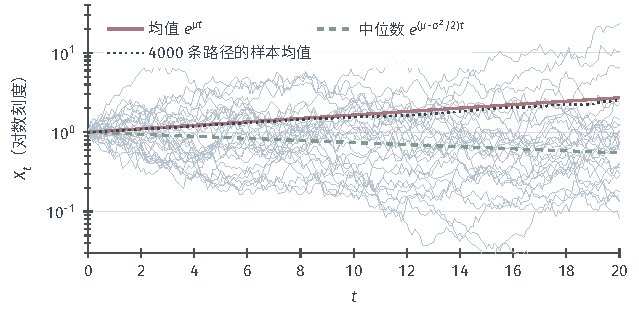
\includegraphics[width=105mm]{figures/03-optimization-evolution-and-signals/02-processes-and-trajectory-evolution/tikz/ctsp-gbm-mean-median/figure.pdf}
  \caption{几何Brownian运动的均值与中位数（纵轴为对数刻度）。$\mu=0.05$，$\sigma=0.4$，$X_0=1$，由显式解在网格上精确生成，固定随机种子。细线是$4000$条路径中的前$30$条；红线为均值$e^{\mu t}$，绿虚线为中位数$e^{(\mu-\sigma^2/2)t}$，点线为$4000$条路径的样本均值。路径主要沿下降的中位数分布，均值由少数大值决定。}
  \label{fig:ctsp-gbm-mean-median}
\end{figure}

\paragraph{Ornstein--Uhlenbeck过程}
第二个基本模型描述带回复力的波动：状态偏离平衡位置时被线性地拉回，同时受到强度恒定的噪声。
\begin{equation}
  \mathrm dX_t=-\lambda X_t\,\mathrm dt+\sigma\,\mathrm dW_t,\qquad\lambda>0 .
  \label{eq:ctsp-ou}
\end{equation}
这是\term{Ornstein--Uhlenbeck过程}（Ornstein--Uhlenbeck process），简称OU过程。求解时像常微分方程一样乘积分因子$e^{\lambda t}$。对$V(t,x)=e^{\lambda t}x\in C^{2,1}$用Itô公式，$\partial_tV=\lambda e^{\lambda t}x$，$\partial_xV=e^{\lambda t}$，$\partial_{xx}V=0$，所以
\[
  \mathrm d\bigl(e^{\lambda t}X_t\bigr)=\lambda e^{\lambda t}X_t\,\mathrm dt+e^{\lambda t}(-\lambda X_t\,\mathrm dt+\sigma\,\mathrm dW_t)=\sigma e^{\lambda t}\,\mathrm dW_t .
\]
二阶修正为零，因为$V$关于$x$是线性的。积分得
\begin{equation}
  X_t=e^{-\lambda t}X_0+\sigma\int_0^te^{-\lambda(t-s)}\,\mathrm dW_s .
  \label{eq:ctsp-ou-solution}
\end{equation}
设$X_0$平方可积且独立于$W$。随机积分的被积函数是确定的，由上一节的结论它是均值零、方差$\sigma^2\int_0^te^{-2\lambda(t-s)}\,\mathrm ds$的高斯变量，于是
\begin{equation}
  \mathbb EX_t=e^{-\lambda t}\mathbb EX_0,\qquad
  \operatorname{Var}(X_t)=e^{-2\lambda t}\operatorname{Var}(X_0)+\frac{\sigma^2}{2\lambda}\bigl(1-e^{-2\lambda t}\bigr).
  \label{eq:ctsp-ou-moments}
\end{equation}
对$s\leq t$，把式~\eqref{eq:ctsp-ou-solution}从$s$开始重写，$X_t=e^{-\lambda(t-s)}X_s+\sigma\int_s^te^{-\lambda(t-r)}\,\mathrm dW_r$，后一项独立于$\mathcal F_s$，所以$\operatorname{Cov}(X_s,X_t)=e^{-\lambda(t-s)}\operatorname{Var}(X_s)$：记忆按速率$\lambda$指数消退。

两个机制在式~\eqref{eq:ctsp-ou-moments}中清楚分开：回复力使初值的均值与方差按$e^{-\lambda t}$、$e^{-2\lambda t}$衰减，持续的噪声不断注入新的方差，二者平衡于$\sigma^2/(2\lambda)$。若初值确定或为与$W$独立的高斯变量，$X_t$本身是高斯的；初值分布取$\mathcal N(0,\sigma^2/(2\lambda))$时，所有时刻的分布都相同。图~\ref{fig:ctsp-ou-envelope}画出从$X_0=3$出发的路径束：均值曲线指数回落，均值加减两倍标准差的包络逐渐并入稳态带。单条路径并不趋于零，它在稳态带内持续波动。

\begin{figure}[htbp]
  \centering
  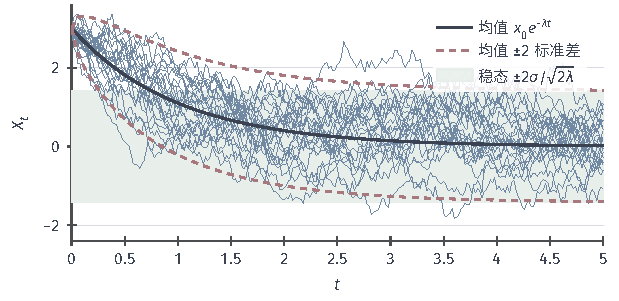
\includegraphics[width=105mm]{figures/03-optimization-evolution-and-signals/02-processes-and-trajectory-evolution/tikz/ctsp-ou-envelope/figure.pdf}
  \caption{OU过程的路径束与矩包络。$\lambda=1$，$\sigma=1$，$X_0=3$；$25$条路径按精确高斯转移在步长$0.01$的网格上生成，固定随机种子。黑线为均值$3e^{-t}$，红虚线为均值$\pm2$倍标准差，绿色带为稳态$\pm2\sigma/\sqrt{2\lambda}$。分布收敛到稳态，路径本身继续波动。}
  \label{fig:ctsp-ou-envelope}
\end{figure}

\paragraph{线性加性噪声系统}
OU过程的推导可以推广到向量情形：
\begin{equation}
  \mathrm d\bm X_t=(\bm A_t\bm X_t+\bm c_t)\,\mathrm dt+\bm G_t\,\mathrm d\bm W_t ,
  \label{eq:ctsp-linear-sde}
\end{equation}
其中$\bm A_t\in\mathbb R^{d\times d}$、$\bm c_t\in\mathbb R^d$、$\bm G_t\in\mathbb R^{d\times m}$都是确定的局部可积函数（$\bm G$局部平方可积），初值$\bm X_0$平方可积且独立于$\bm W$。记$\bm\Phi(t,s)$为齐次方程$\dot{\bm x}=\bm A_t\bm x$的状态转移矩阵（第~\ref{chap:ordinary-differential-equations}章），常系数时$\bm\Phi(t,s)=e^{(t-s)\bm A}$。对$\bm\Phi(0,t)\bm X_t$使用乘积法则~\eqref{eq:ctsp-product-rule}：确定的因子$\bm\Phi(0,t)$有限变差，交叉变差为零，并且$\partial_t\bm\Phi(0,t)=-\bm\Phi(0,t)\bm A_t$，漂移中的$\bm A_t\bm X_t$项正好抵消。积分后乘回$\bm\Phi(t,0)$，
\begin{equation}
  \bm X_t=\bm\Phi(t,0)\bm X_0+\int_0^t\bm\Phi(t,s)\bm c_s\,\mathrm ds+\int_0^t\bm\Phi(t,s)\bm G_s\,\mathrm d\bm W_s .
  \label{eq:ctsp-linear-sde-solution}
\end{equation}
最后一项称为随机卷积。

均值$\bm m_t$与协方差$\bm P_t$可以由路径表达式取矩得到，也可以直接由Itô公式推出。后一种做法对$\widetilde{\bm X}=\bm X-\bm m$的外积用乘积法则：漂移部分给出$\bm A\bm P+\bm P\bm A^\top$，二次协变差给出$\bm G\bm G^\top$，随机积分项在二阶矩有限时期望为零。于是
\begin{equation}
  \dot{\bm m}_t=\bm A_t\bm m_t+\bm c_t,\qquad
  \dot{\bm P}_t=\bm A_t\bm P_t+\bm P_t\bm A_t^\top+\bm G_t\bm G_t^\top .
  \label{eq:ctsp-moment-equations}
\end{equation}
第一项传播已有的不确定性，第二项持续注入新的不确定性。若$\bm A$为常矩阵且所有特征值实部为负，$\bm P_t$趋于Lyapunov方程$\bm A\bm P+\bm P\bm A^\top+\bm G\bm G^\top=\bm0$的唯一解。

关于分布形状需要单独说明。若初值是确定向量，或是与$\bm W$独立的高斯向量，式~\eqref{eq:ctsp-linear-sde-solution}的每个分量都是独立高斯对象的线性组合与$L^2$极限，所以任意有限个时刻的状态联合高斯，矩方程~\eqref{eq:ctsp-moment-equations}就完全决定了分布。初值不是高斯时，$\bm X_t$一般也不是高斯的，均值与协方差只是部分摘要。由状态的带噪观测推断状态，即Kalman滤波，留给第~\ref{chap:state-space-estimation}章。

\begin{example}[受噪声驱动的阻尼振子]
  \label{ex:ctsp-damped-oscillator}
  位置$q$与速度$p$满足$\mathrm dq=p\,\mathrm dt$，$\mathrm dp=(-q-p)\,\mathrm dt+\sigma\,\mathrm dW$：弹簧把位置拉回，摩擦使速度衰减，噪声只直接作用在速度上。此时$\bm A=\begin{pmatrix}0&1\\-1&-1\end{pmatrix}$，$\bm G=(0,\sigma)^\top$。$\bm A$的特征值为$(-1\pm\mathrm i\sqrt3)/2$，实部为负。设稳态协方差$\bm P=\begin{pmatrix}p_{1,1}&p_{1,2}\\p_{1,2}&p_{2,2}\end{pmatrix}$，Lyapunov方程的三个分量给出$2p_{1,2}=0$、$p_{2,2}-p_{1,1}-p_{1,2}=0$、$-2(p_{1,2}+p_{2,2})+\sigma^2=0$，解得$\bm P=\frac{\sigma^2}2\bm I$。噪声只进入速度，位置却得到同样大小的方差，并且稳态下位置与速度不相关。
\end{example}

\subsection{跳跃驱动的状态方程}
\label{sec:ctsp-jump-sde}

\paragraph{事件之间连续演化，事件处更新}
加入速率$\lambda$的Poisson驱动$N$，并规定$\bm W$、$N$与初值相互独立，滤过由三者的历史生成。方程
\begin{equation}
  \mathrm d\bm X_t=\bm b(\bm X_{t-})\,\mathrm dt+\bm\sigma(\bm X_{t-})\,\mathrm d\bm W_t+\bm\gamma(\bm X_{t-})\,\mathrm dN_t
  \label{eq:ctsp-jump-sde}
\end{equation}
的含义仍是积分方程，跳跃项按式~\eqref{eq:ctsp-counting-integral}逐事件累计。解要求是右连续有左极限的适应过程。系数在跳前状态$\bm X_{t-}$处取值，这保证跳跃积分的被积过程可预测；在连续部分，$\bm X_{t-}$与$\bm X_t$只在可数个时刻不同，对$\mathrm dt$与$\mathrm d\bm W$积分没有区别。

这个方程有一个直观的构造。设到达时刻为$T_1<T_2<\cdots$。在$[0,T_1)$上解扩散方程$\mathrm d\bm X=\bm b\,\mathrm dt+\bm\sigma\,\mathrm d\bm W$；在$T_1$处令$\bm X_{T_1}=\bm X_{T_1-}+\bm\gamma(\bm X_{T_1-})$；再从这一新状态出发解扩散方程直到$T_2$，如此继续。若扩散部分满足定理~\ref{thm:ctsp-sde-existence}或定理~\ref{thm:ctsp-nonexplosion}的条件，$\bm\gamma$是有限值的可测函数，有限时段内又只有有限个事件，这一有限次拼接就给出存在且唯一的解。

同一个模型也可以用补偿驱动写出。代入$\mathrm dN=\mathrm d\widetilde N+\lambda\,\mathrm dt$，
\[
  \mathrm d\bm X_t=\bigl[\bm b(\bm X_{t-})+\lambda\bm\gamma(\bm X_{t-})\bigr]\mathrm dt+\bm\sigma(\bm X_{t-})\,\mathrm d\bm W_t+\bm\gamma(\bm X_{t-})\,\mathrm d\widetilde N_t .
\]
补偿形式的漂移多出$\lambda\bm\gamma$，表示跳跃的平均效果；如果只把$\mathrm dN$换成$\mathrm d\widetilde N$而不改漂移，描述的就是另一个模型。

\begin{example}[散粒噪声]
  \label{ex:ctsp-shot-noise}
  考虑$\mathrm dX=-X_{t-}\,\mathrm dt+\sigma\,\mathrm dW_t+c\,\mathrm dN_t$：状态连续泄漏，受到连续的小扰动，并在每个事件时刻增加$c$。均值$m_t=\mathbb EX_t$满足$\dot m=-m+\lambda c$，长期趋于$\lambda c$。对$X^2$使用跳跃Itô公式~\eqref{eq:ctsp-jump-ito}，每次事件使平方增加$(x+c)^2-x^2=2cx+c^2$，所以
  \[
    \frac{\mathrm d}{\mathrm dt}\mathbb EX_t^2=-2\,\mathbb EX_t^2+\sigma^2+\lambda(2cm_t+c^2).
  \]
  稳态下$\mathbb EX^2=\frac12(\sigma^2+2\lambda^2c^2+\lambda c^2)$，减去$m^2=\lambda^2c^2$，得到稳态方差$\frac12(\sigma^2+\lambda c^2)$。连续噪声贡献$\sigma^2$，跳跃贡献$\lambda c^2$，即单位时间内跳幅平方的平均累计量，与第~\ref{sec:ctsp-compensation}节的可预测二阶累计一致。
\end{example}

\paragraph{仍需检查的条件与主线之外的对象}
存在性与不爆炸仍需逐项检查。连续系数要满足上述增长或Lyapunov条件；跳幅$\bm\gamma$若增长很快，单次跳跃可以把状态送到很远的地方，矩估计需要对跳幅加线性增长条件；若事件强度依赖状态并且可以无界增长，有限时间内就可能发生无穷多次事件，上面的有限拼接论证不再适用。状态依赖的有界强度$\lambda(\bm x)\leq\bar\lambda$可以用稀释法构造，第~\ref{sec:ctsp-jump-simulation}节在模拟时说明。

有限时段内无穷多次小跳跃的Lévy驱动、以及状态本身是空间场的随机偏微分方程，都超出本章主线。前者需要用跳跃测度代替逐事件求和，后者需要把第~\ref{chap:partial-differential-equations}章的弱解理论与随机积分结合；它们沿用本章的可预测性与补偿思想，但存在性与正则性需要另外的工具。
